\section{Implementation}

\begin{frame}{Implementation}
    \begin{center}
        Integration of DeepSpeed optimizations into the Open Catalyst Project.
        \vspace{0.5cm}
    \end{center}

    \begin{columns}
        \centering
        \begin{column}{0.5\textwidth}
            \centering
            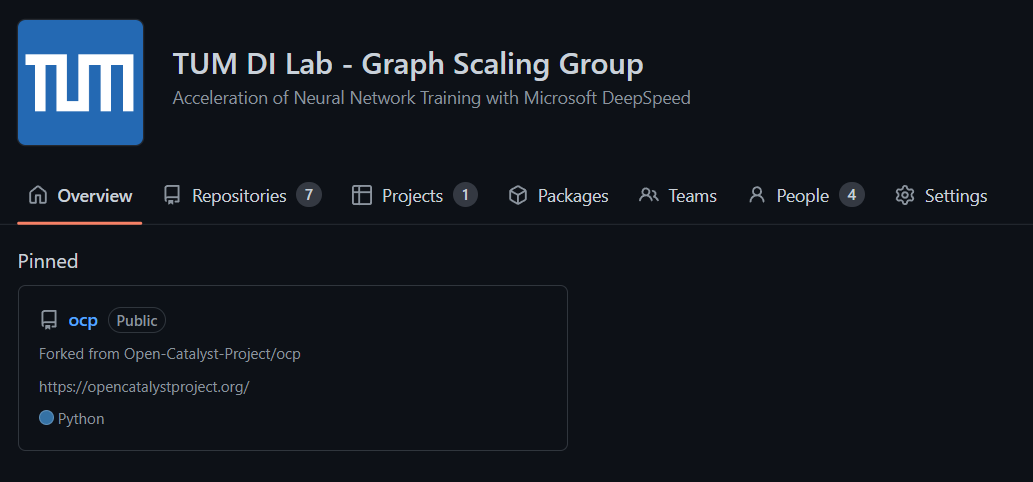
\includegraphics[width=0.9\textwidth]{figures/ocp-branch.png}
            Our code is available on GitHub\footnotemark
        \end{column} 

        \begin{column}{0.5\textwidth}
            \textbf{Integrated Features:}

            \begin{itemize}
                \item \textcolor{tum-green}{\ding{51}} Mixed-Precision Training
                \item \textcolor{tum-green}{\ding{51}} Zero Redundancy Optimizer (ZeRO)
                \item \textcolor{tum-green}{\ding{51}} Offloading Optimizations
            \end{itemize}
        \end{column} 
    \end{columns}
    \footnotetext{\url{https://github.com/TUM-DI-Lab-Graph-Scaling/ocp}}
\end{frame}

\begin{frame}{Mixed Precision}
    Mixed precision training uses lower bit floating point types for model params, gradients 
    and optimizer states

    \begin{small}
        \begin{center}
            \begin{tabular}{|c|c|}
                \hline
                \textbf{Advantages \color{tum-green}\ding{51}} & \textbf{Disadvantages \color{red}\ding{55}} \\
                \hline
                Less memory required & Over/Underflows \\
                Less memory bandwith used & Loss-scaling necessary \\
                Faster CUDA operations & \\
                \hline
            \end{tabular}
        \end{center}
    \end{small} 

    \begin{figure}[H]

    \tikzset{
        bit/.style={
            shape=rectangle,
            draw=tum-gray,
            minimum width=0.4cm,
            minimum height=0.5cm,
            inner sep=0.5
        }
    }

    \centering
    \begin{subfigure}{0.5\textwidth}
        \centering
        
        \begin{tikzpicture}[scale=0.8, transform shape]
            \node[bit, fill=tum-light-green] (0) at (0,0) {\textcolor{tum-dark-green}{\tiny$\boldsymbol{0}$}};
            \node[bit, fill=tum-lighter-blue] (1) at (0.4,0) {\textcolor{tum-dark-blue}{\tiny$\boldsymbol{0}$}};
            \node[bit, fill=tum-lighter-blue] (2) at (0.8,0) {\textcolor{tum-dark-blue}{\tiny$\boldsymbol{1}$}};
            \node[bit, fill=tum-lighter-blue] (3) at (1.2,0) {\textcolor{tum-dark-blue}{\tiny$\boldsymbol{0}$}};
            \node[bit, fill=tum-lighter-blue] (4) at (1.6,0) {\textcolor{tum-dark-blue}{\tiny$\boldsymbol{1}$}};
            \node[bit, fill=tum-lighter-blue] (5) at (2,0) {\textcolor{tum-dark-blue}{\tiny$\boldsymbol{1}$}};
            \node[bit, fill=tum-light-orange] (6) at (2.4,0) {\textcolor{tum-orange}{\tiny$\boldsymbol{0}$}};
            \node[bit, fill=tum-light-orange] (7) at (2.8,0) {\textcolor{tum-orange}{\tiny$\boldsymbol{0}$}};
            \node[bit, fill=tum-light-orange] (8) at (3.2,0) {\textcolor{tum-orange}{\tiny$\boldsymbol{0}$}};
            \node[bit, fill=tum-light-orange] (9) at (3.6,0) {\textcolor{tum-orange}{\tiny$\boldsymbol{0}$}};
            \node[bit, fill=tum-light-orange] (10) at (4,0) {\textcolor{tum-orange}{\tiny$\boldsymbol{0}$}};
            \node[bit, fill=tum-light-orange] (11) at (4.4,0) {\textcolor{tum-orange}{\tiny$\boldsymbol{1}$}};
            \node[bit, fill=tum-light-orange] (12) at (4.8,0) {\textcolor{tum-orange}{\tiny$\boldsymbol{1}$}};
            \node[bit, fill=tum-light-orange] (13) at (5.2,0) {\textcolor{tum-orange}{\tiny$\boldsymbol{1}$}};
            \node[bit, fill=tum-light-orange] (14) at (5.6,0) {\textcolor{tum-orange}{\tiny$\boldsymbol{0}$}};
            \node[bit, fill=tum-light-orange] (15) at (6,0) {\textcolor{tum-orange}{\tiny$\boldsymbol{0}$}};
    
            \node[bit, draw=black] (bit) at (0,0) {};
            \node[bit, draw=black, minimum width=2cm] (exponent) at (1.2,0) {};
            \node[bit, draw=black, minimum width=4cm] (exponent) at (4.2,0) {};
    
            \node[] (sign) at (0,0.7) {\tiny \textbf{\textcolor{tum-dark-green}{sign}}};
            \node[] (1bit) at (0,0.45) {\tiny \textcolor{tum-dark-green}{(1 bit)}};
            \node[] (exponent) at (1.2,0.7) {\tiny \textbf{\textcolor{tum-dark-blue}{exponent}}};
            \node[] (8bit) at (1.2,0.45) {\tiny \textcolor{tum-dark-blue}{(5 bits)}};
            \node[] (fraction) at (4.2,0.7) {\tiny \textbf{\textcolor{tum-orange}{fraction}}};
            \node[] (7bit) at (4.2,0.45) {\tiny \textcolor{tum-orange}{(10 bits)}};
        \end{tikzpicture}
        \caption*{\scriptsize FP16}

    \end{subfigure}%
    ~
    \begin{subfigure}{0.5\textwidth}
        \centering

        \begin{tikzpicture}[scale=0.8, transform shape]
            \node[bit, fill=tum-light-green] (0) at (0,0) {\textcolor{tum-dark-green}{\tiny$\boldsymbol{0}$}};
            \node[bit, fill=tum-lighter-blue] (1) at (0.4,0) {\textcolor{tum-dark-blue}{\tiny$\boldsymbol{0}$}};
            \node[bit, fill=tum-lighter-blue] (2) at (0.8,0) {\textcolor{tum-dark-blue}{\tiny$\boldsymbol{1}$}};
            \node[bit, fill=tum-lighter-blue] (3) at (1.2,0) {\textcolor{tum-dark-blue}{\tiny$\boldsymbol{0}$}};
            \node[bit, fill=tum-lighter-blue] (4) at (1.6,0) {\textcolor{tum-dark-blue}{\tiny$\boldsymbol{1}$}};
            \node[bit, fill=tum-lighter-blue] (5) at (2,0) {\textcolor{tum-dark-blue}{\tiny$\boldsymbol{1}$}};
            \node[bit, fill=tum-lighter-blue] (6) at (2.4,0) {\textcolor{tum-dark-blue}{\tiny$\boldsymbol{0}$}};
            \node[bit, fill=tum-lighter-blue] (7) at (2.8,0) {\textcolor{tum-dark-blue}{\tiny$\boldsymbol{0}$}};
            \node[bit, fill=tum-lighter-blue] (8) at (3.2,0) {\textcolor{tum-dark-blue}{\tiny$\boldsymbol{0}$}};
            \node[bit, fill=tum-light-orange] (9) at (3.6,0) {\textcolor{tum-orange}{\tiny$\boldsymbol{0}$}};
            \node[bit, fill=tum-light-orange] (10) at (4,0) {\textcolor{tum-orange}{\tiny$\boldsymbol{0}$}};
            \node[bit, fill=tum-light-orange] (11) at (4.4,0) {\textcolor{tum-orange}{\tiny$\boldsymbol{1}$}};
            \node[bit, fill=tum-light-orange] (12) at (4.8,0) {\textcolor{tum-orange}{\tiny$\boldsymbol{1}$}};
            \node[bit, fill=tum-light-orange] (13) at (5.2,0) {\textcolor{tum-orange}{\tiny$\boldsymbol{1}$}};
            \node[bit, fill=tum-light-orange] (14) at (5.6,0) {\textcolor{tum-orange}{\tiny$\boldsymbol{0}$}};
            \node[bit, fill=tum-light-orange] (15) at (6,0) {\textcolor{tum-orange}{\tiny$\boldsymbol{0}$}};
    
            \node[bit, draw=black] (bit) at (0,0) {};
            \node[bit, draw=black, minimum width=3.2cm] (exponent) at (1.8,0) {};
            \node[bit, draw=black, minimum width=2.8cm] (exponent) at (4.8,0) {};
    
            \node[] (sign) at (0,0.7) {\tiny \textbf{\textcolor{tum-dark-green}{sign}}};
            \node[] (1bit) at (0,0.45) {\tiny \textcolor{tum-dark-green}{(1 bit)}};
            \node[] (exponent) at (1.8,0.7) {\tiny \textbf{\textcolor{tum-dark-blue}{exponent}}};
            \node[] (8bit) at (1.8,0.45) {\tiny \textcolor{tum-dark-blue}{(8 bits)}};
            \node[] (fraction) at (4.8,0.7) {\tiny \textbf{\textcolor{tum-orange}{fraction}}};
            \node[] (7bit) at (4.8,0.45) {\tiny \textcolor{tum-orange}{(7 bits)}};
        \end{tikzpicture}
        \caption*{\scriptsize Bfloat16}

    \end{subfigure}

    \caption{\footnotesize Comparison of the FP16 and the Bfloat 16 formats.}
    
\end{figure}
\end{frame}

\begin{frame}{Zero Redundancy Optimizer (ZeRO)}
    \begin{figure}[H]
    \centering

    \tikzset{
        gpu/.style={
            shape=rectangle, 
            draw, 
            minimum width=1.8cm,
            minimum height=2.5cm
        },
        data/.style={
            preaction={fill,tum-light-gray},
            shape=rectangle, 
            draw, 
            minimum width=1.8cm, 
            minimum height=0.7cm,
            pattern color=tum-gray,
            pattern=grid
        },
        model/.style={
            preaction={fill,tum-lighter-blue},
            shape=rectangle,
            draw,
            minimum height=0.5cm,
            pattern color=tum-light-blue,
            pattern=grid
        },
        gradient/.style={
            preaction={fill,tum-light-green},
            shape=rectangle,
            draw,
            minimum height=0.5cm,
            pattern color=tum-green,
            pattern=grid
        },
        optimizer/.style={
            preaction={fill,tum-light-orange},
            shape=rectangle,
            draw,
            minimum height=1.5cm,
            pattern color=tum-orange,
            pattern=grid
        },
        empty/.style={
            preaction={fill,tum-lighter-gray},
            shape=rectangle,
            draw,
            minimum width=1.8cm,
            pattern color=tum-light-gray,
            pattern=grid
        }
    }

    \begin{subfigure}[t]{0.5\textwidth}
        \centering
        \begin{tikzpicture}

            \node[gpu, label={\scriptsize GPU $0$}] (0) at (0,0) {};
            \node[gpu, label={\scriptsize GPU $1$}] (1) at (2,0) {};
            \node[gpu, label={\scriptsize GPU $m\!-\!1$}] (n-1) at (4.5,0) {};
            \node[data, label=left:\tiny Data] (0d) at (0,-1.7) {\scriptsize $\mathcal{D}_0$};
            \node[data] (1d) at (2,-1.7) {\scriptsize $\mathcal{D}_1$};
            \node[data] (n-1d) at (4.5,-1.7) {\scriptsize $\mathcal{D}_{m-1}$};
            \draw[dotted, thick] (3,0) -- (3.51,0);
            \draw[dotted, thick] (3,-1.7) -- (3.51,-1.7);
    
            \node[model, minimum width=1.8cm, label=left:\tiny \textcolor{tum-dark-blue}{Model}] (0m) at (0,1) {};
            \node[gradient, minimum width=1.8cm, label=left:\tiny \textcolor{tum-dark-green}{Gradient}] (0g) at (0,0.5) {};
            \node[optimizer, minimum width=1.8cm, label=left:\tiny \textcolor{tum-orange}{Optimizer}] (0o) at (0,-0.5) {};
    
            \node[model, minimum width=1.8cm] (0m) at (2,1) {};
            \node[gradient, minimum width=1.8cm] (0g) at (2,0.5) {};
            \node[optimizer, minimum width=1.8cm] (0o) at (2,-0.5) {};
    
            \node[model, minimum width=1.8cm] (0m) at (4.5,1) {};
            \node[gradient, minimum width=1.8cm] (0g) at (4.5,0.5) {};
            \node[optimizer, minimum width=1.8cm] (0o) at (4.5,-0.5) {};

        \end{tikzpicture}
        \caption*{$\qquad \qquad$\scriptsize \textbf{Stage 0: Standard data parallelism}}
    \end{subfigure}\hspace*{1.4em}%
    ~
    \begin{subfigure}[t]{0.45\textwidth}
        \centering
        \begin{tikzpicture}

            \node[gpu, label={\scriptsize GPU $0$}] (0) at (0,0) {};
            \node[gpu, label={\scriptsize GPU $1$}] (1) at (2,0) {};
            \node[gpu, label={\scriptsize GPU $m\!-\!1$}] (n-1) at (4.5,0) {};
            \node[data] (0d) at (0,-1.7) {\scriptsize $\mathcal{D}_0$};
            \node[data] (1d) at (2,-1.7) {\scriptsize $\mathcal{D}_1$};
            \node[data] (n-1d) at (4.5,-1.7) {\scriptsize $\mathcal{D}_{m-1}$};
            \draw[dotted, thick] (3,0) -- (3.51,0);
            \draw[dotted, thick] (3,-1.7) -- (3.51,-1.7);
    
            \node[model, minimum width=1.8cm] (0m) at (0,1) {};
            \node[gradient, minimum width=1.8cm] (0g) at (0,0.5) {};
            \node[empty, minimum height=1.5cm] (0e) at (0,-0.5) {};
            \node[optimizer, minimum width=0.4cm] (0o) at (-0.7,-0.5) {};
    
            \node[model, minimum width=1.8cm] (0m) at (2,1) {};
            \node[gradient, minimum width=1.8cm] (0g) at (2,0.5) {};
            \node[empty, minimum height=1.5cm] (0e) at (2,-0.5) {};
            \node[optimizer, minimum width=0.4cm] (0o) at (1.7,-0.5) {};
    
            \node[model, minimum width=1.8cm] (0m) at (4.5,1) {};
            \node[gradient, minimum width=1.8cm] (0g) at (4.5,0.5) {};
            \node[empty, minimum height=1.5cm] (0e) at (4.5,-0.5) {};
            \node[optimizer, minimum width=0.4cm] (0o) at (5.2,-0.5) {};

        \end{tikzpicture}
        \caption*{\scriptsize \textbf{ZeRO stage 1}}
    \end{subfigure}

    %\vspace*{0.5em}

    \begin{subfigure}[t]{0.5\textwidth}
        \centering
        \begin{tikzpicture}

            \node[gpu, label={\scriptsize GPU $0$}] (0) at (0,0) {};
            \node[gpu, label={\scriptsize GPU $1$}] (1) at (2,0) {};
            \node[gpu, label={\scriptsize GPU $m\!-\!1$}] (n-1) at (4.5,0) {};
            \node[data, label=left:\tiny Data] (0d) at (0,-1.7) {\scriptsize $\mathcal{D}_0$};
            \node[data] (1d) at (2,-1.7) {\scriptsize $\mathcal{D}_1$};
            \node[data] (n-1d) at (4.5,-1.7) {\scriptsize $\mathcal{D}_{m-1}$};
            \draw[dotted, thick] (3,0) -- (3.51,0);
            \draw[dotted, thick] (3,-1.7) -- (3.51,-1.7);
    
            \node[model, minimum width=1.8cm, label=left:\tiny \textcolor{tum-dark-blue}{Model}] (0m) at (0,1) {};
            \node[empty, minimum height=2cm] (0e) at (0,-0.25) {};
            \node[gradient, minimum width=0.4cm, label=left:\tiny \textcolor{tum-dark-green}{Gradient}] (0g) at (-0.7,0.5) {};
            \node[optimizer, minimum width=0.4cm, label=left:\tiny \textcolor{tum-orange}{Optimizer}] (0o) at (-0.7,-0.5) {};
    
            \node[model, minimum width=1.8cm] (0m) at (2,1) {};
            \node[empty, minimum height=2cm] (0e) at (2,-0.25) {};
            \node[gradient, minimum width=0.4cm] (0g) at (1.7,0.5) {};
            \node[optimizer, minimum width=0.4cm] (0o) at (1.7,-0.5) {};
    
            \node[model, minimum width=1.8cm] (0m) at (4.5,1) {};
            \node[empty, minimum height=2cm] (0e) at (4.5,-0.25) {};
            \node[gradient, minimum width=0.4cm] (0g) at (5.2,0.5) {};
            \node[optimizer, minimum width=0.4cm] (0o) at (5.2,-0.5) {};

        \end{tikzpicture}
        \caption*{$\qquad \qquad$\scriptsize \textbf{ZeRO stage 2}}
    \end{subfigure}\hspace*{1.4em}%
    ~
    \begin{subfigure}[t]{0.45\textwidth}
        \centering
        \begin{tikzpicture}

            \node[gpu, label={\scriptsize GPU $0$}] (0) at (0,0) {};
            \node[gpu, label={\scriptsize GPU $1$}] (1) at (2,0) {};
            \node[gpu, label={\scriptsize GPU $m\!-\!1$}] (n-1) at (4.5,0) {};
            \node[data] (0d) at (0,-1.7) {\scriptsize $\mathcal{D}_0$};
            \node[data] (1d) at (2,-1.7) {\scriptsize $\mathcal{D}_1$};
            \node[data] (n-1d) at (4.5,-1.7) {\scriptsize $\mathcal{D}_{m-1}$};
            \draw[dotted, thick] (3,0) -- (3.51,0);
            \draw[dotted, thick] (3,-1.7) -- (3.51,-1.7);
    
            \node[empty, minimum height=2.5cm] (0e) at (0,0) {};
            \node[model, minimum width=0.4cm] (0m) at (-0.7,1) {};
            \node[gradient, minimum width=0.4cm] (0g) at (-0.7,0.5) {};
            \node[optimizer, minimum width=0.4cm] (0o) at (-0.7,-0.5) {};
    
            \node[empty, minimum height=2.5cm] (0e) at (2,0) {};
            \node[model, minimum width=0.4cm] (0m) at (1.7,1) {};
            \node[gradient, minimum width=0.4cm] (0g) at (1.7,0.5) {};
            \node[optimizer, minimum width=0.4cm] (0o) at (1.7,-0.5) {};
    
            \node[empty, minimum height=2.5cm] (0e) at (4.5,0) {};
            \node[model, minimum width=0.4cm] (0m) at (5.2,1) {};
            \node[gradient, minimum width=0.4cm] (0g) at (5.2,0.5) {};
            \node[optimizer, minimum width=0.4cm] (0o) at (5.2,-0.5) {};

        \end{tikzpicture}
        \caption*{\scriptsize \textbf{ZeRO stage 3}}
    \end{subfigure}
    \vspace*{-0.5em}

    \captionsetup{width=\dimexpr\textwidth-1.5cm\relax}
    \caption{GPU memory utilization with different stages of ZeRO activated.
    The data $\mathcal{D}$ is distributed evenly among the $m$ GPUs into 
    $\mathcal{D}_0, \dots, \mathcal{D}_{m-1}$.}
\end{figure}
\end{frame}

\begin{frame}{Offloading Optimizations}
    Deepspeed Offload-Engine determines optimizer states and gradients which can be 
    computed on CPU using RAM or NVMe. \\~\\ 

    \begin{columns}
        \begin{column}{0.5\textwidth}
            \vspace{-0.75cm}
            \begin{center}
                \begin{small}
                    The engine optimizes tensor
                    allocation w.r.t:
                    \begin{itemize}
                        \bitem CPU-GPU computation overhead
                        \bitem Communication costs
                        \bitem Memory savings
                    \end{itemize}
                \end{small}
            \end{center}
        
        \end{column}
        \begin{column}{0.5\textwidth}
            \begin{center}
                \begin{figure}[H]
                    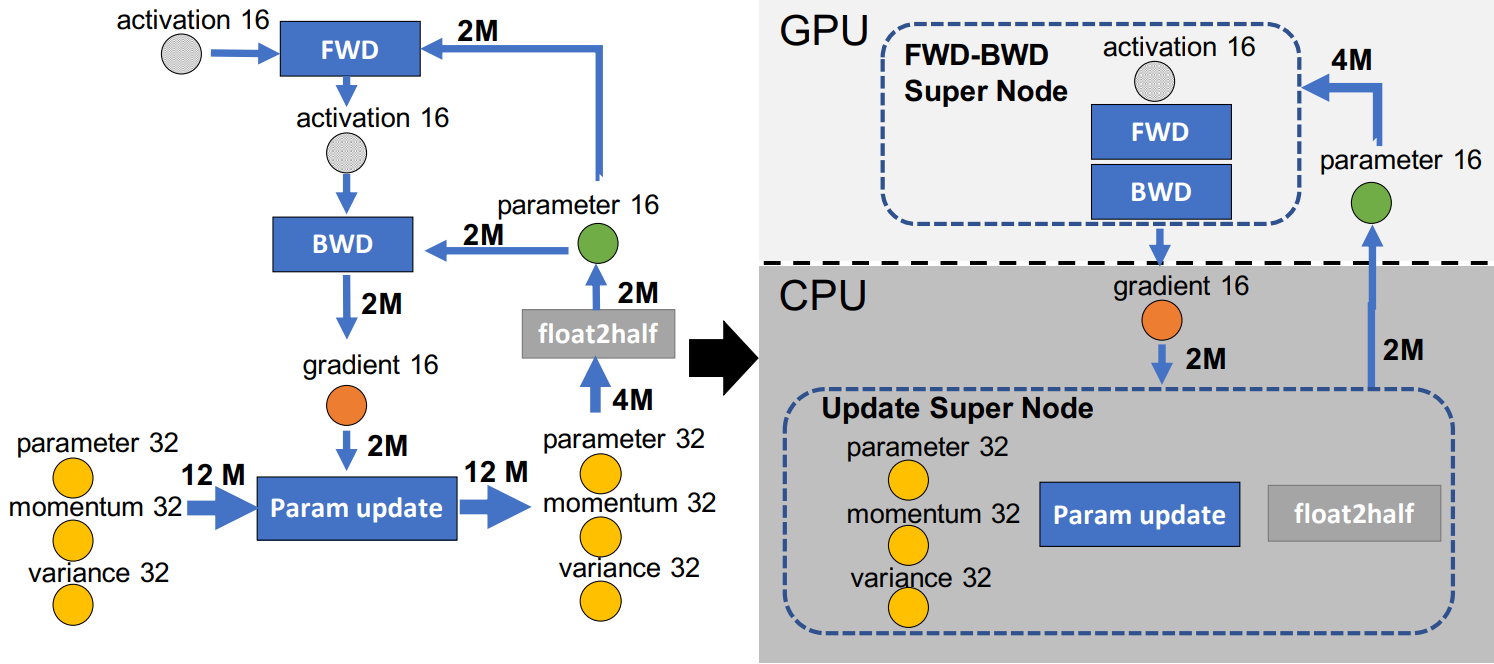
\includegraphics[scale=.17]{figures/data_flow_graph.png}
                    \caption*{\scriptsize Dataflow graph of a neural network. 
                    Right side: CPU and GPU partitions \footnotemark}
                \end{figure}
            \end{center}
        \end{column}
    \end{columns}
    \footnotetext{\fullcite{DBLP:journals/corr/abs-2101-06840}}
\end{frame}

\begin{frame}{Deepspeed Configuration}
    \centering
    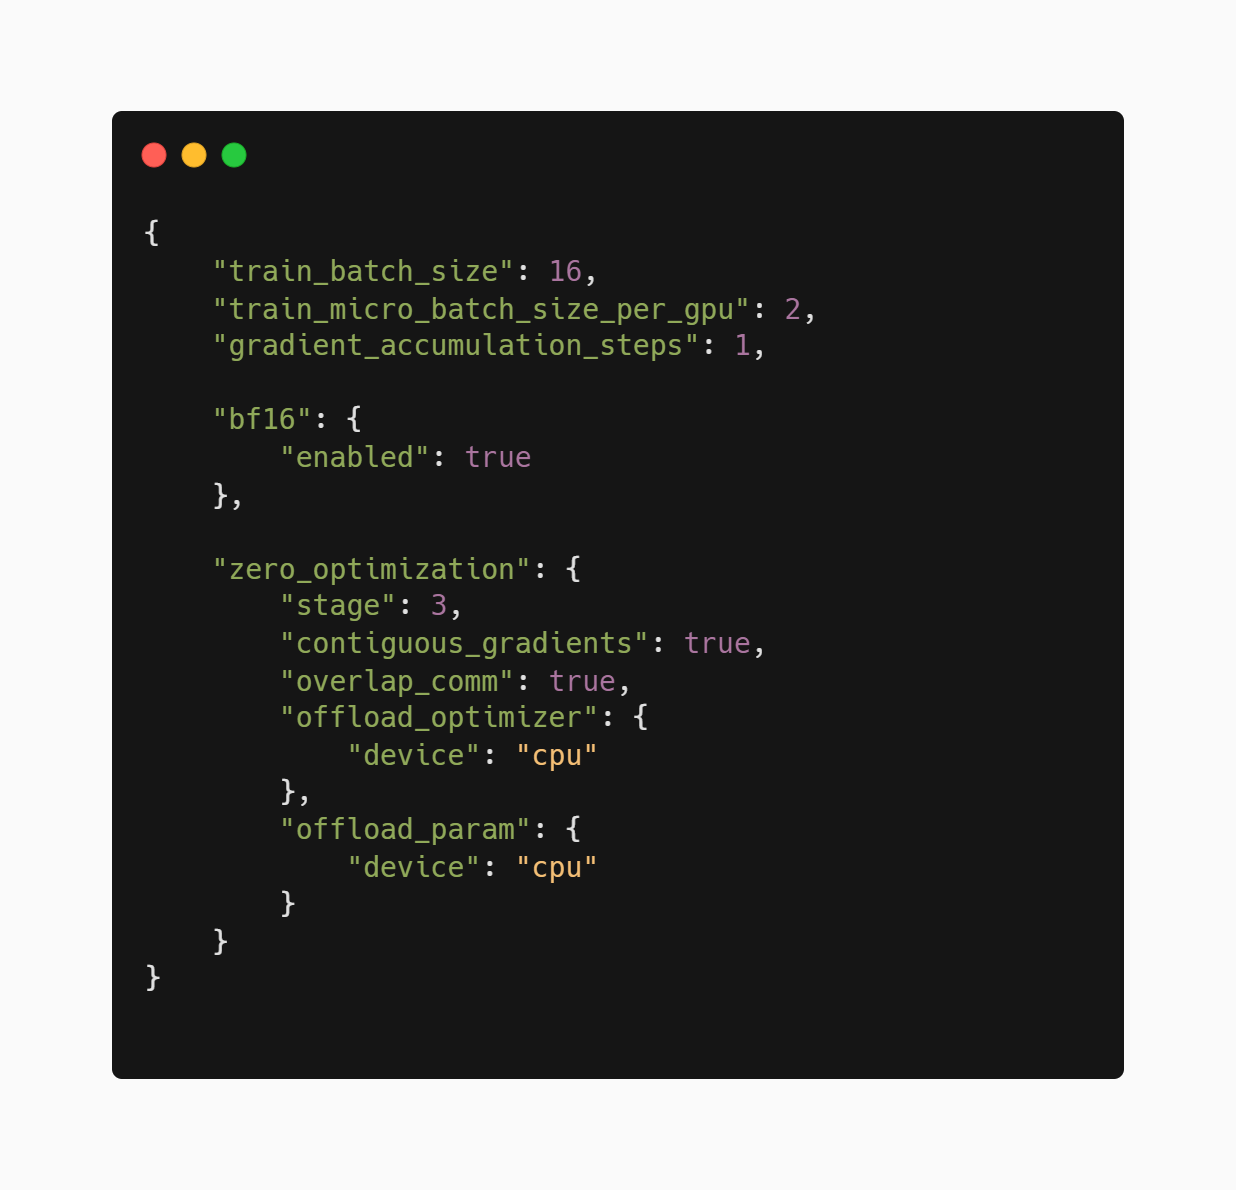
\includegraphics[scale=.18]{figures/ds_config.png}
\end{frame}